% THIS IS SIGPROC-SP.TEX - VERSION 3.1
% WORKS WITH V3.2SP OF ACM_PROC_ARTICLE-SP.CLS
% APRIL 2009
%
% Questions regarding SIGS should be sent to
% Adrienne Griscti ---> griscti@acm.org
%
% Questions/suggestions regarding the guidelines, .tex and .cls files, etc. to
% Gerald Murray ---> murray@hq.acm.org
%
% For tracking purposes - this is V3.1SP - APRIL 2009
%
% Copied from https://github.com/heathermiller/papers-documents/tree/master/rem2013

\documentclass{support/acm_proc_article-sp}
\usepackage{listings}
\usepackage{url}
\usepackage{support/bcprules}
\usepackage{support/prooftree}
\usepackage{support/math}
\usepackage{multicol}
\usepackage{caption}
\usepackage{subcaption}
\usepackage[normalem]{ulem}
\usepackage{color}
\usepackage{graphicx}
\usepackage{hyperref}

\renewcommand{\thesubsection}{\thesection.\alph{subsection}}

\definecolor{blue}{rgb}{0,0,0.5}
\definecolor{red}{rgb}{0.6,0,0}
\definecolor{green}{rgb}{0,0.5,0}
\definecolor{grey}{rgb}{0.2,0.2,0.2}

\lstdefinelanguage{Python}{
keywords={typeof, null, catch, switch, in, int, str, float, self, from, import},
keywordstyle=\color{blue}\bfseries,
ndkeywords={boolean, throw, import},
ndkeywords={return, class, if ,elif, endif, while, do, else, True, False , catch, def},
ndkeywordstyle=\color{blue}\bfseries,
identifierstyle=\color{grey},
sensitive=false,
comment=[l]{\#},
morecomment=[s]{/*}{*/},
commentstyle=\color{green}\ttfamily,
stringstyle=\color{green}\ttfamily,
}

\lstset{language=Python}

\clubpenalty = 10000
\widowpenalty = 10000
\displaywidowpenalty = 10000

% Remove copyright space
\makeatletter
\def\@copyrightspace{\relax}
\makeatother

% comments and notes
\newcommand{\comment}[1]{}
\newcommand{\note}[1]{{\bf $\clubsuit$ #1 $\spadesuit$}}
\newcommand{\ifreport}[1]{#1}
%\newcommand{\ifreport}[1]{}

\newcommand{\todo}{{\bf \colorbox{red}{\color{white}TODO:}}}
\newcommand{\ie}{{\em i.e.,~}}
\newcommand{\eg}{{\em e.g.,~}}
\newcommand{\term}[1]{\mbox{\texttt{#1}}}
\newcommand{\itl}[1]{\mbox{\textit{#1}}}

% commas and semicolons
\newcommand{\comma}{,\,}
\newcommand{\commadots}{\comma \ldots \comma}
\newcommand{\semi}{;\mbox{;};}
\newcommand{\semidots}{\semi \ldots \semi}

% spacing
\newcommand{\gap}{\quad\quad}
\newcommand{\biggap}{\quad\quad\quad}
\newcommand{\nextline}{\\ \\}
\newcommand{\htabwidth}{0.5cm}
\newcommand{\tabwidth}{1cm}
\newcommand{\htab}{\hspace{\htabwidth}}
\newcommand{\tab}{\hspace{\tabwidth}}
\newcommand{\linesep}{\ \hrulefill \ \smallskip}

\newcommand{\sectionline}{%
\nointerlineskip \vspace{\baselineskip}%
\hspace{\fill}\rule{0.5\linewidth}{.7pt}\hspace{\fill}%
\par\nointerlineskip \vspace{\baselineskip}
}

% figures
\newcommand{\figurebox}[1]
{\fbox{\begin{minipage}{\textwidth}
           #1 \medskip
\end{minipage}}}
\newcommand{\twofig}[3]
{\begin{figure*}[t]
     #3\ \hrulefill\
        \caption{\label{#1}#2}
\end{figure*}}
\newcommand{\boxfig}[3]
{\begin{figure*}
     \figurebox{#3\caption{\label{#1}#2}}
\end{figure*}}
\newcommand{\figref}[1]
{Figure~\ref{#1}}

% arrays
\newcommand{\ba}{\begin{array}}
\newcommand{\ea}{\end{array}}
\newcommand{\bda}{\[\ba}
\newcommand{\eda}{\ea\]}
\newcommand{\ei}{\end{array}}
\newcommand{\bcases}{\left\{\begin{array}{ll}}
\newcommand{\ecases}{\end{array}\right.}

\pagenumbering{arabic}
\begin{document}

    \title{Data Mining and Matrices (FSS18) \\ Assignment 1: Singular Value Decomposition}

    \numberofauthors{1}
    \author{
    \alignauthor
    Steffen Schmitz\\
    \affaddr{University of Mannheim}\\
    \affaddr{stefschm@mail.uni-mannheim.de}
    }

    \maketitle

    %%%%%%%%%%%%%%%%%%%%%%%%%%%%%%%%%%%%%%%%%%%%%%%%%%%%
    %%
    %% 1) Intuition on SVD
    %%
    %%%%%%%%%%%%%%%%%%%%%%%%%%%%%%%%%%%%%%%%%%%%%%%%%%%%

    \section{Intuition on SVD}

    %%%%%%%%%%%%%%%%%%%%%%%%%%%%%%%%%%%%%%%%%%%%%%%%%%%%
    %%
    %% 1.a) Manual Estimation
    %%
    %%%%%%%%%%%%%%%%%%%%%%%%%%%%%%%%%%%%%%%%%%%%%%%%%%%%

    \subsection{Manual Estimation}
    \label{subsec:manest}

    \textbf{Task.} Try to manually obtain the rank of each of the following matrices, as well as its singular values,
    and the left and right singular vectors corresponding to the non-zero singular values.
    Do this by "looking" at the data and try to infer how the (compact) SVD needs to look like.

    We start the exercise by determining the rank of each matrix and try to guess the SVD afterwards.
    The row or column rank of a matrix is the maximum number of linearly independent rows or columns, respectively.
    Except for matrix $\mathbf{M}_2$, all matrices are symmetric ($\mathbf{M}_n = \mathbf{M}_n^T$), which means that
    the row and column rank are equal to each other.

    The rows and columns of $\mathbf{M}_2$ are similar and are all linear combinations of each other.
    We determine that the rank of $\mathbf{M}_2$ is 1.

    For the first matrix $\mathbf{M}_1$ we learn that all rows and columns
    are linear combinations of the first one (either by multiplication with 1 or 0).
    Therefore, we conclude that the rank $r$ of $\mathbf{M}_1$ is 1.

    We can make the same argument for matrix $\mathbf{M}_3$.
    Its rank $r$ is 1, too.

    $\mathbf{M}_4$ is the first matrix where we can't compute all rows and columns as a linear combination of another
    one.
    The first three rows and columns and the last two rows and columns are linear combinations of each other.
    The rank $r$ of $\mathbf{M}_4$ is 2.
    We estimate the rank $r$ of $\mathbf{M}_6$ to be also 2 for the same reason.

    The remaining matrix $\mathbf{M}_5$ should have a rank $r$ or 3, because the first two rows and the last two rows
    are linearly dependent and the third row is independent of all the others.

    The singular value decomposition of a matrix $\mathbf{A}$ with $n$ rows and $m$ columns is
    \begin{equation*}
        \mathbf{A} = \mathbf{U}\mathbf{\Sigma}\mathbf{V}^T
    \end{equation*}
    where the superscript $T$ indicates the transpose of matrix $\mathbf{V}$ \cite[p. 49]{skillicorn2007}.
    We obtain the compact SVD by truncating $\mathbf{U}$ and $\mathbf{V}^T$ to $r$ columns and rows, respectively.
    $\mathbf{\Sigma}$ will be a diagonal $r \mbox{ x } r$ matrix.

    For the first three matrices with rank $r = 1$, we expect $\mathbf{\Sigma}$ to be only a scalar value and the singular
    vectors $\mathbf{U}$ and $\mathbf{V}$ to have the shape $5 \mbox{ x } 1$.

    As already said, we expect the rank $r$ of $\mathbf{M}_4$ to be 2.
    This means that we have a $2 \mbox{ x } 2$ matrix for the diagonal matrix $\mathbf{\Sigma}$ and $5 \mbox{ x } 2$
    singular vectors for the compact SVD\@.

    For an overview of estimated compact SVDs have a look at the Jupyter Notebook that was handed in together with
    this document.
    Usually, the singular vectors would have orthogonal unit vectors as their rows and columns, but, unfortunately,
    I was unable to estimate those correctly.

    %%%%%%%%%%%%%%%%%%%%%%%%%%%%%%%%%%%%%%%%%%%%%%%%%%%%
    %%
    %% 1.b) Actual SVD
    %%
    %%%%%%%%%%%%%%%%%%%%%%%%%%%%%%%%%%%%%%%%%%%%%%%%%%%%

    \subsection{Actual SVD}

    \textbf{Task.} Compute the SVD (e.g., using R's \lstinline{svd} function) and compare.
    Have you been correct?

    Again, the computed SVDs are included in the corresponding Jupyter Notebook.
    In general, the assumptions made in Section \ref{subsec:manest} seem to hold.
    The first three matrices have a rank of 1 and the values the estimated values also seem related to the actual, computed
    values.
    As already mentioned, we haven't normalized the vectors, which explains the deviation.

    The same observation holds for matrix $\mathbf{M}_4$ which has a rank of 2 and 2 non-zero singular values.

    For the matrix $\mathbf{M}_5$ we see the first deviation between expected and actual results.
    We estimated the rank of $\mathbf{M}_5$ to be equal to 3, which would correspond to 3 non-zero singular values.
    \begin{equation}
        \mathbf{\Sigma}_5 = \begin{pmatrix}
            3.56 & 0 & 0    & 0              & 0 \\
            0    & 2 & 0    & 0              & 0 \\
            0    & 0 & 0.56 & 0              & 0 \\
            0    & 0 & 0    & 3\cdot10^{-17} & 0 \\
            0    & 0 & 0    & 0              & 0 \\
        \end{pmatrix}
        \label{eq:sigma5}
    \end{equation}
    In Equation \ref{eq:sigma5} we can see that R computes 4 non-zero singular values, which shows that the actual
    rank of matrix $\mathbf{M}_5$ is 4.
    Nevertheless, we can argue that $3\cdot10^{-17}$ effectively is zero and has little to no influence on the result
    if we reconstruct the matrix.
    Our approximation from \ref{subsec:manest} is, therefore, also reasonable for $\mathbf{M}_5$.

    Last but not least, we estimated a rank of 2 for matrix $\mathbf{M}_{6}$.
    The singular values again indicate a higher rank, 5 in this case, but all singular values after the second are
    very close to zero ($\sigma_{i > 2} < 1\cdot10^{-15}$).
    If we apply the same argument as for matrix $\mathbf{M}_5$ we conclude, that a rank of 2 is also sufficient to
    approximate $\mathbf{M}_{6}$ almost perfectly.

    The estimated compact SVD for matrix $\mathbf{M}_5$ and $\mathbf{M}_6$ are also reasonable, if we ignore
    normalization.

    %%%%%%%%%%%%%%%%%%%%%%%%%%%%%%%%%%%%%%%%%%%%%%%%%%%%
    %%
    %% 1.c) Rank-1 Approximation
    %%
    %%%%%%%%%%%%%%%%%%%%%%%%%%%%%%%%%%%%%%%%%%%%%%%%%%%%

    \subsection{Rank-1 Approximation}

    \textbf{Task.} How does the best rank-1 approximation look like?
    Is it "intuitive"?

    According to the \textsc{Eckart-Young-Theorem}, the \emph{best} rank-$k$ approximation of a matrix is given by
    the rank-$k$ truncated SVD\@.
    Therefore, we can compute the best rank-1 approximation by multiplying the first column of $\mathbf{U}$ with the
    first singular value and the first row of $\mathbf{V}^T$.

    We do not take the matrices $\mathbf{M}_{1}$, $\mathbf{M}_{2}$ and $\mathbf{M}_{3}$ into account, because their rank
    already is 1 and the best rank-1 approximation is the matrix itself.

    For matrix $\mathbf{M}_{4}$ we observe that the upper left part is reconstructed perfectly, while the four entries
    in the lower right corner stay at zero.
    Following our estimation from Section \ref{subsec:manest} this is also intuitive.
    We can observe two sets of linear dependent rows in the original matrix and reconstruct only one of them perfectly
    with the rank-1 approximation.

    The result is less obvious for the matrices $\mathbf{M}_{5}$ and $\mathbf{M}_{6}$.
    We observe that the approximation is unable to reconstruct the basic shape of matrix $\mathbf{M}_{5}$.
    We would expect the four entries in the top right and bottom left of the matrix to be closer to 0, while all
    other values in the matrix approximate 1, but, all values that are apart from the middle row and column are the same.
    It seems that the SVD emphasizes that the middle row and column are also all 1s.

    The approximation of matrix $\mathbf{M}_{6}$ seems much better.
    The lowest value is assigned to the entry in the middle of the matrix which corresponds to the only 0 value in the
    original matrix.
    Values on the middle row and column are still smaller than 1 and diverge from the other approximated entries, but
    the structure of matrix $\mathbf{M}_{6}$ can be derived from the approximation.

    %%%%%%%%%%%%%%%%%%%%%%%%%%%%%%%%%%%%%%%%%%%%%%%%%%%%
    %%
    %% 1.d) SVD Approximation in R
    %%
    %%%%%%%%%%%%%%%%%%%%%%%%%%%%%%%%%%%%%%%%%%%%%%%%%%%%

    \subsection{SVD Approximation in R}

    \textbf{Task.} How many non-zero singular values does $\mathbf{M}_{6}$ have, i.e.\@, what is the rank
    of $\mathbf{M}_{6}$?
    How many non-zero singular values are reported by R?
    Discuss!

    Computing the SVD in WolframAlpha\footnote{\href{http://www.wolframalpha.com/input/?i=svd+\%7B\%7B1,1,1,1,1\%7D,\%7B1,1,1,1,1\%7D,\%7B1,1,0,1,1\%7D,\%7B1,1,1,1,1\%7D,\%7B1,1,1,1,1\%7D\%7D}{http://www.wolframalpha.com}}
    provides us with two non-zero singular values $d \approx (4.83, 0.83, 0, 0, 0)$ for the decomposition of $\mathbf{M}_{6}$, which fits to the rank
    of 2 for the matrix, that we computed with R's \lstinline{rankMetrix} function.

    With R's \lstinline{svd} function we obtain $d \approx (4.83, 0.83, 2.42\cdot10^{-16}, 3\cdot10^{-18}, 2.13\cdot10^{-50})$
    as the singular values which effectively corresponds to a rank of 5.

    At this point we can apply the same argument as in Section \ref{subsec:manest}, namely, that all singular values after
    the second are effectively zero and it is likely that they are caused by issues in the float representation in R\@.

    This assumptions is confirmed by computing the rank-2 approximation of matrix $\mathbf{M}_{6}$, which effectively
    returns the original matrix (again, taking float representation issues into account).

    %%%%%%%%%%%%%%%%%%%%%%%%%%%%%%%%%%%%%%%%%%%%%%%%%%%%
    %%
    %% 2) The SVD on Weather Data
    %%
    %%%%%%%%%%%%%%%%%%%%%%%%%%%%%%%%%%%%%%%%%%%%%%%%%%%%

    \section{The SVD on Weather Data}

    %%%%%%%%%%%%%%%%%%%%%%%%%%%%%%%%%%%%%%%%%%%%%%%%%%%%
    %%
    %% 2.a) Computing z-scores
    %%
    %%%%%%%%%%%%%%%%%%%%%%%%%%%%%%%%%%%%%%%%%%%%%%%%%%%%

    \subsection{Computing z-scores}
    \label{subsec:z-scores}

    \textbf{Task.} Normalize the data to $z$-scores.
    Considering the data we are using, are the assumptions for normalizing the data reasonable?

    We normalize the data using R's \lstinline{scale} function that takes a matrix, normalizes and centers it.
    First, it computes the mean of each column and subtracts it from each element and afterwards divides them by the
    column mean.

    This transforms a distribution with any mean and any standard deviation to the normal distribution
    $\mathcal{N}(0, 1)$.
    The $z$-score transformation implicitly assumes that the data follows a standard distribution, which means that we need
    to confirm that each column's distribution follows approximately a bell shape.

    From the plots in the corresponding Jupyter Notebook we learn that this is the case and the application of
    $z$-scores on the climate set is reasonable.

    % skip b, because it only is about implementation
    \stepcounter{subsection}

    %%%%%%%%%%%%%%%%%%%%%%%%%%%%%%%%%%%%%%%%%%%%%%%%%%%%
    %%
    %% 2.c) Interpreting the SVD
    %%
    %%%%%%%%%%%%%%%%%%%%%%%%%%%%%%%%%%%%%%%%%%%%%%%%%%%%

    \subsection{Interpreting the SVD}
    \label{subsec:interpret-svd}

    \textbf{Task.} Plot each of the first 5 columns of $\mathbf{U}$.
    Use the longitude and latitude of each data point as the $x$ and $y$ coordinates, respectively, and the
    corresponding entry in the left singular vector to color each point.
    Can you interpret the result?

    Figure \ref{fig:2c-1} shows the plot for the first column of $\mathbf{U}$.
    \begin{figure}[!htbp]
        \centering
        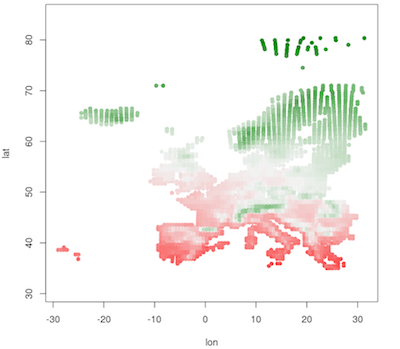
\includegraphics[width=8cm]{images/2c-1.png}
        \caption{Plot for first column of $\mathbf{U}$}
        \label{fig:2c-1}
    \end{figure}
    We can see that the continental regions in the South and the West are red, while the North, Iceland and the region
    around the Alps are green.
    The colors are the strongest in the South and in the North and blurred in the middle.
    Comparing this chart to typical climate landscapes of Europe, we conclude that the red zones correspond to overall
    warmer regions and the green zones to overall colder regions in Europe.

    The second column is displayed in Figure \ref{fig:2c-2}.
    \begin{figure}[!htbp]
        \centering
        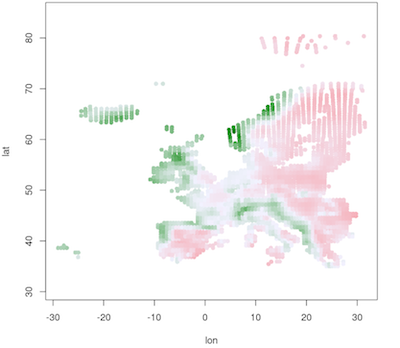
\includegraphics[width=8cm]{images/2c-2.png}
        \caption{Plot for second column of $\mathbf{U}$}
        \label{fig:2c-2}
    \end{figure}
    We can see that the West Coast and the region around the Alps are greenish, while the continental regions are more likely
    to be red.

    If we compare it with the monthly precipitation in Europe in the month of April
    (Figure \ref{fig:april-precip-europe}\footnote{http://www.mappedplanet.com/karten/klima/april\_nied-eu.png}) we
    can see that there is a strong correlation between those charts.
    \begin{figure}[!htbp]
        \centering
        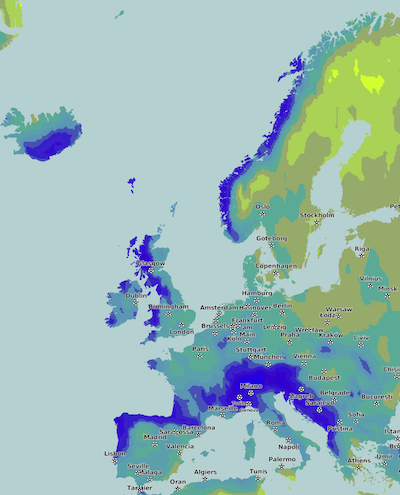
\includegraphics[width=6cm]{images/april-precip-europe.png}
        \caption{Monthly precipitation in Europe in April}
        \label{fig:april-precip-europe}
    \end{figure}
    Hence, the green zones in Figure \ref{fig:2c-2} correspond to regions with more rain, while the red zones show
    drier regions.
    We still have to keep in mind that Figure \ref{fig:2c-2} contains data for the whole year, while Figure \ref{fig:april-precip-europe}
    displays only a single month.

    Nevertheless, we can assume that the second column indicates whether a specific regions experiences more
    precipitation or less.

    For the third column of the left singular values displayed in Figure \ref{fig:2c-3} we get large red areas in regions
    that are close or adjacent to the sea.
    \begin{figure}[!htbp]
        \centering
        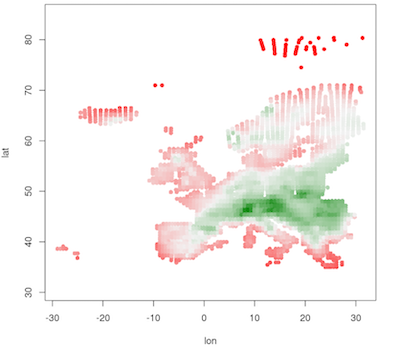
\includegraphics[width=8cm]{images/2c-3.png}
        \caption{Plot for third column of $\mathbf{U}$}
        \label{fig:2c-3}
    \end{figure}
    In this interpretation red regions are closer to the sea, while green regions are further away.

    The fourth column of the matrix $\mathbf{U}$ is depicted in Figure \ref{fig:2c-4}.
    We can see that Spain, the Alps and large parts of Greece have the deepest green, while Great Britain and the northern
    part of central Europe is mostly red.
    \begin{figure}[!htbp]
        \centering
        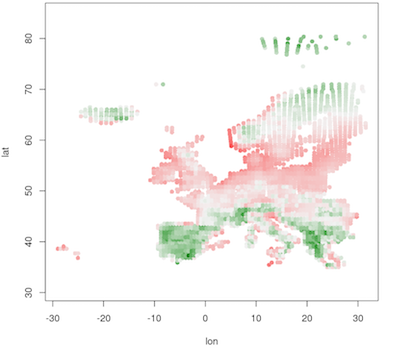
\includegraphics[width=8cm]{images/2c-4.png}
        \caption{Plot for fourth column of $\mathbf{U}$}
        \label{fig:2c-4}
    \end{figure}
    Knowing that the Alps are around the middle of the map and there are multiple mountains in Spain and Greece,
    the coloring in Figure \ref{fig:2c-4} can be compared to the relief
    map in Europe shown in Figure \ref{fig:relief-europe}\footnote{\href{http://www.vidiani.com/maps/maps\_of\_europe/detailed\_physical\_and\_relief\_map\_of\_europe.jpg}{http://www.vidiane.com/map\_of\_europe.jpg}}.
    \begin{figure}[!htbp]
        \centering
        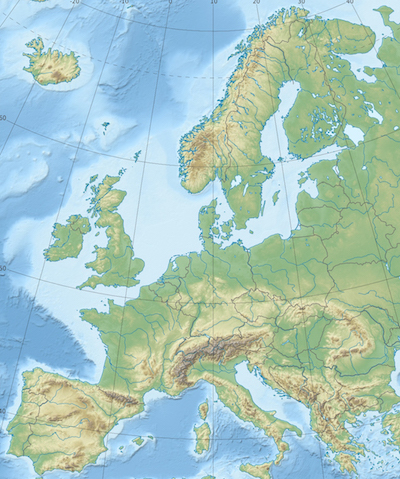
\includegraphics[width=6cm]{images/relief-europe.png}
        \caption{Relief map of Europe}
        \label{fig:relief-europe}
    \end{figure}
    From the comparison we infer that green regions correspond to elevated regions on the map and red regions signify
    proximity to the sea.
    We know that the weather and the precipitation in the mountains is different than in other regions and this seems
    also relevant for the reconstruction of our original matrix.

    We conclude the analysis with an interpretation of the fifth column of the left singular vector $\mathbf{U}$.
    \begin{figure}[!htbp]
        \centering
        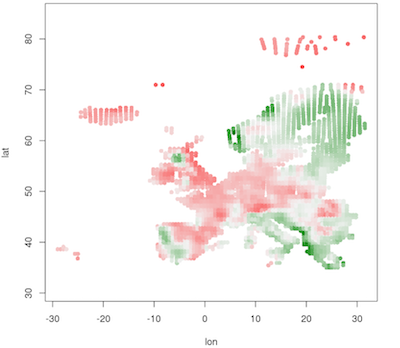
\includegraphics[width=8cm]{images/2c-5.png}
        \caption{Plot for fifth column of $\mathbf{U}$}
        \label{fig:2c-5}
    \end{figure}
    A part of Scotland, Portugal and most parts of Scandinavia and the former Yugoslavia are green, while the rest of
    Europe is mostly colored red.
    Unfortunately, we can not think of any similarity that those regions have and therefore lack an interpretation for
    this map.

    %%%%%%%%%%%%%%%%%%%%%%%%%%%%%%%%%%%%%%%%%%%%%%%%%%%%
    %%
    %% 2.d) Interpreting the SVD
    %%
    %%%%%%%%%%%%%%%%%%%%%%%%%%%%%%%%%%%%%%%%%%%%%%%%%%%%

    \subsection{Interpreting the SVD}

    \textbf{Task.} Plot some scatterplots between the columns of $\mathbf{U}$ using colors to distinguish either their
    North-South or East-West location.
    Can you interpret the results?

    In Section \ref{subsec:interpret-svd} we estimated that the first column of the left singular vector indicates
    the average temperature in each region and the second indicates the precipitation in each region.
    We plot those two columns in Figure \ref{fig:2d-1}.
    \begin{figure}[!htbp]
        \centering
        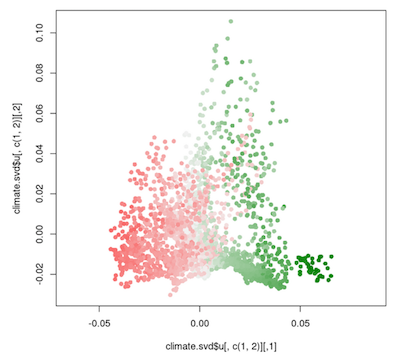
\includegraphics[width=8cm]{images/2d-1.png}
        \caption{Compare first and second column of $\mathbf{U}$}
        \label{fig:2d-1}
    \end{figure}
    On the $x$-axis we see the values for the first column, on the $y$-axis the value of the second column, and the
    color indicates whether the region is in the North or in the South.

    The chart shows that the two groups are clearly separated with regards to the first column.
    This fits the behavior we observed in the previous section, where regions in the South are warmer than in the North.
    For the value of the second column we see that regions with a low values in the first column of $\mathbf{U}$ are
    closer together with regards to the precipitation, while regions with a high value have more variance.

    In Figure \ref{fig:2d-2} we analyze the second and the fifth column of the left singular values.
    The $x$-axis shows the precipitation in Europe and, again, we lack an interpretation for the $y$-axis.
    \begin{figure}[!htbp]
        \centering
        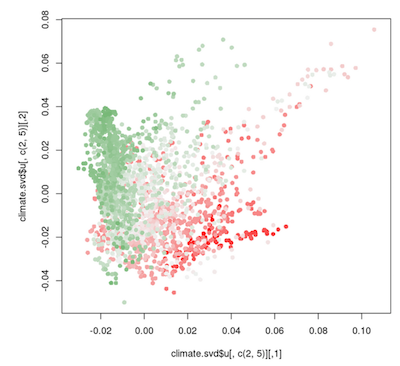
\includegraphics[width=8cm]{images/2d-2.png}
        \caption{Compare second and fifth column of $\mathbf{U}$}
        \label{fig:2d-2}
    \end{figure}
    The colors in Figure \ref{fig:2d-2} indicate the East-West relation of the regions.

    Contrasting this chart with our results from Section \ref{subsec:interpret-svd}, we see that most of the rain falls in
    the East of Europe.
    This is also exemplified by the dense, green cluster for small values of $x$.
    We conclude that almost all of Europe's precipitation takes place in the East.

    %%%%%%%%%%%%%%%%%%%%%%%%%%%%%%%%%%%%%%%%%%%%%%%%%%%%
    %%
    %% 2.e) Rank Selection
    %%
    %%%%%%%%%%%%%%%%%%%%%%%%%%%%%%%%%%%%%%%%%%%%%%%%%%%%

    \subsection{Rank Selection}

    \textbf{Task.} Try the different rank selection methods listed below to decide what would be a good rank for a
    truncated SVD.
    Report the rank each method suggests (and when subjective evaluation is needed, say why you picked your choice).

    The current rank of our climate matrix is 48 and we want to find a lower-rank approximation that reconstructs the
    original matrix as good as possible, while reducing noise and size of the SVD\@.

    \subsubsection{Guttman-Kaiser Criterion}

    The Guttman-Kaiser criterion selects all values $\sigma_i$ where $\sigma_i > 1$.
    Applying this criterion to the singular values of our climate dataset, we obtain a suggested rank of 37.

    \subsubsection{90\% of squared Frobenius norm}

    For the 90\% of squared Frobenius norm criterion we select the singular values in a way that the sum of their squares
    exceeds 90\% of the sum of the squares of all singular values.
    For the climate dataset we only need the first 3 out of the 48 singular values to fulfill this criterion.

    A problem with both the Guttman-Kaiser criterion and the 90\% of squared Frobenius norm are the arbitrary thresholds.
    We might as well select only singular values $\sigma_i > 5$ or expect the truncated SVD to "explain" 85\% of the
    singular values.
    For the reasons stated above, we will not take those into consideration when choosing the rank that we want to
    truncate to.

    \subsubsection{Scree test}

    We plot the singular values in decreasing order and look for a point where the values even out or there is a
    clear drop in the magnitude of the values.
    The plot is shown in Figure \ref{fig:2e-scree}.
    \begin{figure}[!htbp]
        \centering
        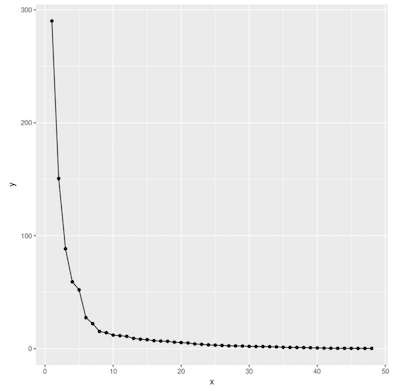
\includegraphics[width=8cm]{images/2e-scree.png}
        \caption{Scree test for weather data SVD.}
        \label{fig:2e-scree}
    \end{figure}

    There is a clear drop after the sixth singular value.
    Therefore, we select rank $k=6$ for the truncation.

    \subsubsection{Entropy-based method}

    We compute each singular values contribution to the Frobenius norm and treat those as probabilities.
    Then we compute the entropy of the resulting vector and select $k$, so that the sum of contributions of the
    first $k$ singular values is bigger than the computed entropy.

    With this method we obtain a recommendation $k=1$.

    \subsubsection{Random flipping of signs}

    We try to select $k$ in a manner that the residual matrix contains mostly or almost only noise.
    Looking at the plotted result, we find to find a small value of $k$ for which the structure of the residual
    matrix is small.
    A good result with a small $k$ is around $k=10$.
    For the implementation and the chart have a look at the attached Jupyter Notebook.

    As the overall value of $k$ we pick the result of the Scree test, which is 6.
    Following the obvious drop in the magnitude in the values there is little ambiguity in the Scree test result.
    Next, we take the results of the entropy-based method and the random-flipping into account, if the Scree test result
    is complicated to interpret or unambiguous.

    %%%%%%%%%%%%%%%%%%%%%%%%%%%%%%%%%%%%%%%%%%%%%%%%%%%%
    %%
    %% 2.f) RMSE and Noise
    %%
    %%%%%%%%%%%%%%%%%%%%%%%%%%%%%%%%%%%%%%%%%%%%%%%%%%%%

    \subsection{RMSE and Noise}

    \textbf{Task.} Create a noisy version of of your normalized climate data by adding i.i.d.\@ Gaussian noise from
    $\mathcal{N}(0, \epsilon^2)$, where $\epsilon$ is a parameter that corresponds to the standard deviation of the noise.
    Do this for various choices of $\epsilon \in [0,2]$.
    Now create a plot with $\epsilon$ on the $x$-axis and the RMSE on the $y$-axis.
    Add a line for the RMSE between the original data and the noisy data.
    For $k \in {1,2,5,10}$, add a line for the RMSE between the rank-$k$ truncated SVD of climate.normal and the rank-$k$
    truncated SVD of climate.noise.
    Discuss the results.

    In Figure \ref{fig:rmse-noise} we display the RMSE between the original data and the noisy data for different truncation
    levels.
    In this case, the truncation with $k=48$ corresponds to the original matrix, because its rank is 48.
    \begin{figure}[!htbp]
        \centering
        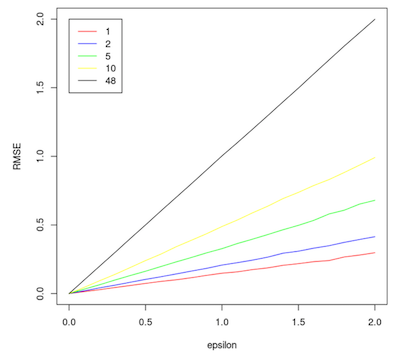
\includegraphics[width=8cm]{images/rmse-noise.png}
        \caption{RMSE and Noise.}
        \label{fig:rmse-noise}
    \end{figure}

    The figure shows that the error between the truncated original matrix and the truncated noisy matrix increases with the
    truncation parameter $k$.
    The SVD behaves exactly as expected in this case, because we assumed that a small rank approximation removes much
    noise, while keeping the most important features.
    If we increase $k$ we also include more of the modeled noise in our reconstruction which leads to poorer results
    with increasing size of $k$.

    %%%%%%%%%%%%%%%%%%%%%%%%%%%%%%%%%%%%%%%%%%%%%%%%%%%%
    %%
    %% 3) Clustering and Visualizing
    %%
    %%%%%%%%%%%%%%%%%%%%%%%%%%%%%%%%%%%%%%%%%%%%%%%%%%%%

    \section{Clustering and Visualizing}

    %%%%%%%%%%%%%%%%%%%%%%%%%%%%%%%%%%%%%%%%%%%%%%%%%%%%
    %%
    %% 3.a) kMeans Result
    %%
    %%%%%%%%%%%%%%%%%%%%%%%%%%%%%%%%%%%%%%%%%%%%%%%%%%%%

    \subsection{kMeans Result}

    \textbf{Task.} Look at the resulting clustering and explain what the clusters may represent.

    The data is clustered with kMeans into 5 clusters.
    In a next step, each region in Europe is colored depending on its cluster so that regions with the same color have similar
    features in the original matrix.
    Figure \ref{fig:kmeans} visualizes the clustering.
    \begin{figure}[!htbp]
        \centering
        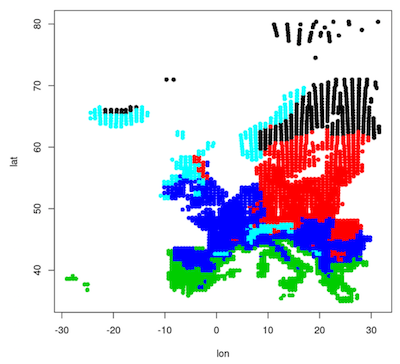
\includegraphics[width=8cm]{images/kmeans.png}
        \caption{kMeans clustering of weather data.}
        \label{fig:kmeans}
    \end{figure}

    Following that the input of the of the clustering corresponds to weather data it is likely that the clusters represent
    different climate zones in Europe, where regions with the same color also have a similar climate.
    This again correlates with the observation that the South has the same cluster.
    Similarly, the continental region and Great Britain share
    a cluster, whereas Scandinavia and the East each have a different cluster.

    If we compare this to a climate map in Europe it is obvious that the green cluster resembles mediterranean
    climate, while the blue cluster is oceanic and the red correlates with a warm continental climate.
    This confirms our assumption.

    %%%%%%%%%%%%%%%%%%%%%%%%%%%%%%%%%%%%%%%%%%%%%%%%%%%%
    %%
    %% 3.b) kMeans and SVD
    %%
    %%%%%%%%%%%%%%%%%%%%%%%%%%%%%%%%%%%%%%%%%%%%%%%%%%%%

    \subsection{kMeans and SVD}
    \label{subsec:kmeans-svd}

    \textbf{Task.} For another visualization of the results, plot the data so that the $x$-axis position comes from the
    first left singular vector, the $y$-axis position comes from the second left singular vector, and the color of each
    point is defined by the cluster identifier.
    Are the clusters well-separated from each other in the plot or are they mixed?
    Do some of the clusters look like outliers?

    The resulting plot is shown in Figure \ref{fig:kmeans-svd}.
    \begin{figure}[!htbp]
        \centering
        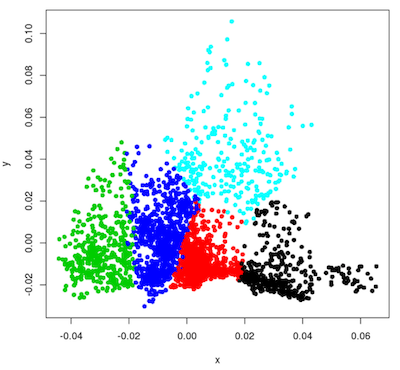
\includegraphics[width=8cm]{images/kmeans-svd.png}
        \caption{SVD analysis with kMeans clustering.}
        \label{fig:kmeans-svd}
    \end{figure}
    The diagram demonstrates that the red, blue and green cluster may also be summarized as a single big cluster,
    as there is no clear separation between the three.
    Comparing this with Figure \ref{fig:kmeans}, we notice that the grouping of the clusters resembles the structure
    of Europe as one big continental region, which confirms the thought that they can also be one big group.

    The other two groups, the black and the blue, are more clearly separated.

    Outliers can most probably be found in the black cluster.
    All values with $x > 0.05$ seem like another cluster that is different from the actual one.
    As a result it may be necessary to increase the number of clusters $k$ to get better results.

    %%%%%%%%%%%%%%%%%%%%%%%%%%%%%%%%%%%%%%%%%%%%%%%%%%%%
    %%
    %% 3.c) Principal Component Analysis
    %%
    %%%%%%%%%%%%%%%%%%%%%%%%%%%%%%%%%%%%%%%%%%%%%%%%%%%%

    \subsection{Principal Component Analysis}

    \textbf{Task.} Compute the PCA scores of the data points for the first $k$ principal components for $k \in { 1, 2, 3 }$,
    thereby reducing dimensionality to $k$.
    Do this using the SVD of the appropriate version of the climate data.
    Repeat the clustering and visualization steps of a) with this new data.
    Did the results change?
    Why do you think the results changed or did not change?

    After computing the PCA for our normalized climate dataset, we plot it the same way as in Section \ref{subsec:kmeans-svd}.
    This results in a similar plot, where the main regions of clusters correspond to each other, yet, there are some
    differences between the two plots.

    One major difference is that the parts of the South, which are close to the mediterranean sea, now share a cluster with
    England and that the region that was previously only in the East expands into much of continental Europe.
    The Alps also get their own cluster in the PCA clustering.

    Actually, I would expect the two charts to be similar, because the only additional assumption that the PCA makes is
    that the data is centered, what was done in Section \ref{subsec:z-scores}.
    From there it is possible to compute the PCA from the SVD results.

    %%%%%%%%%%%%%%%%%%%%%%%%%%%%%%%%%%%%%%%%%%%%%%%%%%%%
    %%
    %% BIBLIOGRAPHY
    %%
    %%%%%%%%%%%%%%%%%%%%%%%%%%%%%%%%%%%%%%%%%%%%%%%%%%%%

    \bibliographystyle{abbrv}
    \bibliography{support/bib}

\end{document}
